\chapter{Problemstellung und Forschungsfrage} \label{cha:Problemstellung}

Die Montage von Rauchmeldern ist ein Prozess in der BRUNATA-METRONA GmbH \& Co. KG, welcher von Mitarbeitern beziehungsweise Dienstleistern regelmäßig durchgeführt wird. Bei der Positionierung der Rauchmelder gibt es eine Reihe von Regeln und Richtlinien, die die Monteure beachten müssen, um eine korrekte Installation zu gewährleisten. 

Diese Regeln sind in einem 83-seitigen \citet{brunata2023handbuch} festgehalten und mit den Vorschriften der entsprechenden DIN-Normen und den Landesbauordnungen der einzelnen Bundesländer abgestimmt. Neben allgemeiner Beschreibungen der Funktionsweise und der Montage von Rauchmeldern enthält das Handbuch auch spezifische Anweisungen zur Positionierung der Rauchmelder in verschiedenen Räumen. Diese Informationen werden in Form von Texten und Abbildungen dargestellt und müssen während des Montageprozesses berücksichtigt werden.


\begin{figure}
\centering
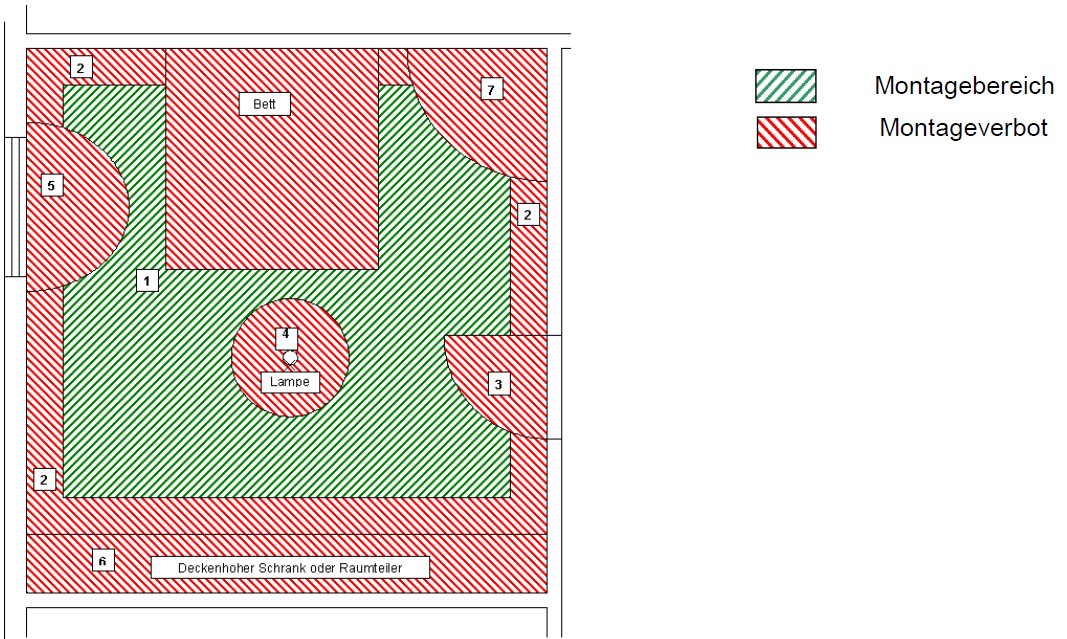
\includegraphics[ width=.8\textwidth ]{Montageanleitung_Wohn-_und_Schlafraeume}
\caption{Montageanleitung für Wohn- und Schlafräume \cite{brunata2023handbuch}\label{fig:Anleitung}}\par
\end{figure}

Die Abbildung~\ref{fig:Anleitung} zeigt eine Montageanleitung für Wohn- und Schlafräume. Auffällig ist, dass der Montagebereich zwar klar definiert ist, die exakte Positionierung des Rauchmelders jedoch nicht explizit angegeben wird. Die Monteure müssen daher die Vorschriften eigenständig interpretieren und entsprechend umsetzen.

Die wichtigsten Regeln für die Montage von Rauchmeldern lassen sich wie folgt zusammenfassen:

\begin{enumerate}
    \item Montage ausschließlich an Decken
    \item Montage möglichst mittig im Raum
    \item 60cm Mindestabstand zu Wänden
    \item 60cm Mindestabstand zu Einrichtungsgegenständen wie deckenhohen Schränken
    \item Montage in Tür- und Fensterbereichen unzulässig
    \item 60cm Mindestabstand zu Deckenlampen
    \item 150cm Mindestabstand zu Decken-, Boden- und Wandöffnungen für Kühl- und Heizungsaus- und -einlässe 
    \item Bei einer Raumfläche von mehr als 60m² sind mehrere Rauchmelder erforderlich
    \item Maximale Raumhöhe von 6m
    \item Bei schrägen Decken ist ein Abstand zur Deckenspitze einzuhalten
\end{enumerate}


Die Missachtung dieser Regeln kann dazu führen, dass die Rauchmelder nicht ordnungsgemäß funktionieren oder im Ernstfall nicht rechtzeitig Alarm schlagen. Dies kann unter Umständen nicht nur rechtliche Konsequenzen nach sich ziehen und somit Reputationsschaden anrichten, sondern auch Menschenleben gefährden. Daher ist es von entscheidender Bedeutung, dass die Monteure die Montageregeln korrekt einhalten und die Rauchmelder gemäß den Vorschriften installieren.

Eine mobile Augmented-Reality-Anwendung, die es den Monteuren ermöglicht, die Montageregeln direkt in der realen Welt zu visualisieren, könnte die Montage von Rauchmeldern effizienter und sicherer gestalten. Die Monteure könnten die Regeln direkt am Montageort einsehen und müssten sich nicht auf ihr Gedächtnis oder das Handbuch verlassen. Dies würde die Wahrscheinlichkeit von Fehlern reduzieren und die Qualität der Installation verbessern.

Die Forschungsfrage, die in dieser Arbeit beantwortet werden soll, lautet daher: \textbf{Wie kann eine Augmented-Reality-Anwendung für mobile Smart-Geräte entwickelt werden, die Monteuren hilft, die korrekten Installationspositionen für Rauchmelder zu visualisieren und so die Einhaltung der Montagevorschriften sowie die Qualität und Effizienz des Installationsprozesses zu verbessern?}

